% document specification
\documentclass[a4paper, 11pt, oneside]{book}
\usepackage[onehalfspacing]{setspace}
\usepackage[left=35mm,right=30mm,top=15mm,bottom=15mm, includeheadfoot, headsep=10mm, footskip=10mm]{geometry}

% unicode
\usepackage[utf8]{inputenc}

% language
\usepackage[english]{babel}

% date
\usepackage[en-US]{datetime2}

% watermark
\usepackage[firstpage]{draftwatermark}

% comments
\usepackage{verbatim}

% tables
\usepackage{booktabs}

% appendix
\usepackage[toc, page]{appendix}

% bibliography
\usepackage[round]{natbib}
\bibliographystyle{plainnat}

% math, equations
%\usepackage{amsmath}
\usepackage{mathtools}

% code listings
\usepackage{listings}
\usepackage{courier}
\usepackage{color}
% define colors for python code
\definecolor{deepblue}{RGB}{0,0,128}
\definecolor{deepgreen}{RGB}{0,100,0}
\definecolor{newgray}{RGB}{105,105,105}

% define code style
\lstset{ %
  backgroundcolor=\color{white},   % choose the background color; you must add \usepackage{color} or \usepackage{xcolor}; should come as last argument
  basicstyle=\footnotesize,        % the size of the fonts that are used for the code
  breakatwhitespace=false,         % sets if automatic breaks should only happen at whitespace
  breaklines=true,                 % sets automatic line breaking
  captionpos=b,                    % sets the caption-position to bottom
  commentstyle=\color{newgray}\itshape,    % comment style
  deletekeywords={...},            % if you want to delete keywords from the given language
  escapeinside={\%*}{*)},          % if you want to add LaTeX within your code
  extendedchars=true,              % lets you use non-ASCII characters; for 8-bits encodings only, does not work with UTF-8
  frame=single,	                   % adds a frame around the code
  keepspaces=true,                 % keeps spaces in text, useful for keeping indentation of code (possibly needs columns=flexible)
  keywordstyle=\color{deepblue}\bfseries,       % keyword style
  language=Python,                 % the language of the code
  morekeywords={self,True, False},            % if you want to add more keywords to the set
  numbers=left,                    % where to put the line-numbers; possible values are (none, left, right)
  numbersep=5pt,                   % how far the line-numbers are from the code
  numberstyle=\tiny\color{black}, % the style that is used for the line-numbers
  rulecolor=\color{black},         % if not set, the frame-color may be changed on line-breaks within not-black text (e.g. comments (green here))
  showspaces=false,                % show spaces everywhere adding particular underscores; it overrides 'showstringspaces'
  showstringspaces=false,          % underline spaces within strings only
  showtabs=false,                  % show tabs within strings adding particular underscores
  stepnumber=1,                    % the step between two line-numbers. If it's 1, each line will be numbered
  stringstyle=\color{deepgreen},     % string literal style
  tabsize=2,	                   % sets default tabsize to 2 spaces
  title=\lstname                   % show the filename of files included with \lstinputlisting; also try caption instead of title
}

\usepackage{fancyhdr}
\usepackage{framed}
\usepackage{mdframed}
\usepackage{multirow}
\usepackage[T1]{fontenc}
\usepackage{amssymb}
\usepackage{thmtools}
\usepackage{setspace}
\usepackage{amsfonts}
\usepackage{graphicx}
\usepackage{graphicx, subfigure}
\usepackage{lmodern}
\usepackage{float}
\usepackage{transparent}
\usepackage[table,xcdraw]{xcolor}
\usepackage{acronym}
\declaretheorem{theorem}
\declaretheorem{example}
\newtheorem{definition}{Definition}[chapter]
\setcounter{tocdepth}{3}
\setcounter{secnumdepth}{3}
\usepackage[final]{pdfpages}

% pdf information
\usepackage[
	pdftitle={Masterthesis Marcus Ritter},
	pdfsubject={Dynamic Order Sourcing Optimization for Online Retail with Deep Reinforcement Learning},
	pdfauthor={Marcus Ritter},
	pdfkeywords={Dynamic Order Sourcing, Online Retail, Machine Learning, Deep Reinforcement Learning, Q-Learning, Neural Network, TensorFlow, Python},
	hidelinks=true
]{hyperref}

\begin{document}

% cover page
\begin{titlepage}
\label{sec:title_page}

% watermark confidential notice
\SetWatermarkText{Non-disclosure notice}
\SetWatermarkScale{0.5}
%\SetWatermarkColor[gray]{0.5}
%\SetWatermarkFontSize{2cm}
%\SetWatermarkAngle{30}


\includegraphics[scale=0.175]{Figures/sap_logo.png}\hfill
\includegraphics[scale=0.4]{Figures/srh_logo.png}\\ 
\vspace{2em}
\begin{center}
\begin{huge}
\begin{onehalfspace}
\textbf{Dynamic Order Sourcing Optimization for Online Retail with Deep Reinforcement Learning}
\end{onehalfspace}
\end{huge}

\vspace{6em}

{\huge Master Thesis}\\

\vspace{1em}

{\LARGE by}\\

\vspace{1em}
\huge{\textbf{Marcus Ritter}}\\

\vspace{1em}
\Large{Matriculation number: 11004061}\\

\vspace{3em}

{\normalsize {\today}}\\

\vspace{2em}

{\Large SRH University Heidelberg}\\
{\Large School of Information, Media and Design}\\
{\Large Degree course ``Applied Computer Science''}\\
{\Large Major field ``Business Computing''}\\

\vspace{3em}

\begin{normalsize}
\makebox{Reviewers}\hspace{3cm}\makebox{Professor Barbara Sprick}\\
\vspace{0.5em}
\makebox{}\hspace{3.95cm}\makebox{Doctor Owen Hickey}\\
\end{normalsize}
\end{center}

\vspace*{\fill}
\end{titlepage}

% second page
\begin{titlepage}
\label{sec:detail_page}

\vspace{2em}
\begin{center}
\begin{LARGE}
\begin{onehalfspace}
\textbf{Dynamic Order Sourcing Optimization for Online Retail with Deep Reinforcement Learning}\\
\end{onehalfspace}
\end{LARGE}

\vspace{1em}
{\LARGE by}\\

\LARGE{Marcus Ritter}\\

\vspace{1em}
\large{Matriculation number: 11004061}\\

\vspace{4em}

\large{Submitted to the School of Information, Media and Design on \today, in partial fulfillment of the requirements for the degree of Master of Science in Applied Computer Science}\\

\end{center}

\vspace{8em}

\begin{flushleft}

\begin{large}
Thesis Advisory Committee
\end{large}

\vspace{3em}

\enspace\dotfill (Internal Supervisor)\\
Professor Barbara Sprick\\
SRH University Heidelberg\\

\vspace{2em}

\enspace\dotfill (Internal Supervisor)\\
Professor Gerd Moeckel\\
SRH University Heidelberg\\

\vspace{2em}

\enspace\dotfill (External Advisor)\\
Doctor Owen Hickey\\
SAP\\

\end{flushleft}

\vspace*{\fill}
\end{titlepage}

% roman page numbering
\pagenumbering{roman}
%\pagenumbering{Roman}
\setcounter{page}{3}

% affidavit
\section*{Affidavit}
\label{sec:affidavit}
\pagestyle{plain}

Herewith I declare:
\begin{itemize}
\item that I have composed the chapters for the Master Thesis for which I am named as the author independently,
\item that I did not use any other sources and additives than the ones specified,
\item that I did not submit this work at any other examination procedure.
\end{itemize}

\begin{verbatim}

\end{verbatim}
\makebox[0.5\textwidth]{Heidelberg,\enspace\hrulefill}   \makebox[0.5\textwidth]{ Signature\enspace\hrulefill}

% restriciton note, nd notice
\section*{Non-disclosure notice}
\label{sec:non-disclosure_notice}

This thesis is subject to a non - publication / disclosure notice as it contains
strictly confidential information of SAP SE. It may not be duplicated, published, or
made available to unauthorized persons, neither in full nor in part, also not in
digital version. Written permission must be obtained from SAP before any
publication of this thesis or before passing it to third parties other than the
relevant university employees, e.g. correctors or the examination board.

\begin{verbatim}

\end{verbatim}
\makebox[0.5\textwidth]{Heidelberg,\enspace\hrulefill}   \makebox[0.5\textwidth]{ Signature\enspace\hrulefill}

% dedication
%\section*{Dedication}
\label{sec:dedication}

Lorem ipsum dolor sit amet, consectetur adipiscing elit, sed do eiusmod tempor incididunt ut labore et dolore magna aliqua. Ut enim ad minim veniam, quis nostrud exercitation ullamco laboris nisi ut aliquip ex ea commodo consequat. Duis aute irure dolor in reprehenderit in voluptate velit esse cillum dolore eu fugiat nulla pariatur. Excepteur sint occaecat cupidatat non proident, sunt in culpa qui officia deserunt mollit anim id est laborum.

% acknowledgement
\section*{Acknowledgement}
\label{sec:acknowledgement}

First and foremost, I would like to thank all my colleagues at SAP with whom I was working in the Retail Omni-Channel Consumer Industries department and especially the manager Simona Dumitru who gave me the opportunity to work on this project. I would also like to thank Owen Hickey and Baris Yalcin for their supervision during the project. I truly appreciate their willingness to answer all my questions, provide input and discuss the project. In addition I would like to thank Professor Barbara Sprick and Professor Gerd Moeckel for their assistance and suggestions throughout the course of this study. It was a pleasure for me to work with all these people.

% abstract
\section*{Abstract}
\label{sec:abstract}

Lorem ipsum dolor sit amet, consectetur adipiscing elit, sed do eiusmod tempor incididunt ut labore et dolore magna aliqua. Ut enim ad minim veniam, quis nostrud exercitation ullamco laboris nisi ut aliquip ex ea commodo consequat. Duis aute irure dolor in reprehenderit in voluptate velit esse cillum dolore eu fugiat nulla pariatur. Excepteur sint occaecat cupidatat non proident, sunt in culpa qui officia deserunt mollit anim id est laborum.

% toc
%\pdfbookmark{\contentsname}{Contents}
\tableofcontents

% list of figures
\listoffigures

% list of tables
\listoftables

% list of listings
\lstlistoflistings

\begin{comment}

%__Abkürzungsverzeichniss__
\newpage
\markboth{Abkürzungsverzeichnis}{} 
\addchap{Abkürzungsverzeichnis} %Abkürzungsverzeichnis 
\vspace{1em} %für etwas Abstand
\begin{acronym}
%Muss Manuell sortiert werden!!!
\acro{BASF}{Badische Anilin- und Soda-Fabrik}
\acro{BU}{Business Unit}
\acro{DWH}{Data-Warehouse}
\acro{DWHS}{Data-Warehouse-System}
\acro{ETL}{Extract Transform Load}
\acro{EV}{Performance Chemicals}
\acro{EV/BS}{Strategy, Innovation Management and R\&D Controlling EV}
\acro{IGC}{International Group of Controlling}
\acro{KPI}{Key Performance Indicator}
\acro{MAT-System}{Mensch/Aufgabe/Technik-System}
\acro{NPV}{Net Present Value}
\acro{OD}{Operating Division}
\acro{ODS}{Operational Data Store}
\acro{OEP}{Object Engineering Process}
\acro{OLAP}{Online Analytical Processing}
\acro{OOAD}{Objektorientierte Analyse und Design}
\acro{ROI}{Return on Investment}
\acro{SBU}{Strategic Business Unit}
\acro{SE}{Societas Europaea}
\acro{UML}{Unified Modeling Language}
\acro{UP}{Unified Process}
\end{acronym}
\pagebreak
%__Definitionsverzeichnis__
\newpage
\renewcommand{\listtheoremname}{Definitionsverzeichnis}
\listoftheorems[ignoreall, show={definition}]

\end{comment}

% header and footer definition
\fancyhead{} 
\lhead{\slshape\nouppercase{\leftmark}}
\chead{}
\rhead{}
\lfoot{}
\cfoot{\thepage}
\rfoot{}
\renewcommand{\headrulewidth}{0.4pt}
\renewcommand{\footrulewidth}{0pt}

% main part of the thesis starts here
\newpage
\setcounter{page}{1}
\pagenumbering{arabic}
\pagestyle{fancy}

% chapter 1 - introduction
\chapter{Introduction} 
\label{sec:chapter1}

\begin{framed}
\textbf{TODO:}
\begin{enumerate}
\item Hinführung zum Thema
\item Praktische, Wissenschaftliche Motivation
\item Problemstellung
\item Eingrenzung der Problemstellung / was ist Teil der Arbeit und was nicht
\item Zielsetzung
\item Methoden und Vorgehen / Welche Methodik wird eingesetzt um die Ziele zu erreichen
\item ML einführen
\item Beiträge der Arbeit
\item Wie die Lösung evaluiert wird
\item Wie man zur Lösung kommt (Inhalt der einzelnen Chapter)
\end{enumerate}
\end{framed}

\section{Motivation}

Today's retail market is quickly changing and holds many challenges for the retailers competing in this business (it). E-commerce or online retailing became absolutely indispensable for the majority of the companies. Accordingly you can see that the share of the sales volume on online retails is increasing every year.


heavily characterized by e-commerce and online retailers. 

Dispite the clasical pure online retailers like Amazon, also traditional retailers (Brick and Mortar retailers) are making their step to e-commerce and start selling their products online.


Like with the change in the dotcom era from normal to online retail now the shift goes to omni-channel retailing. This is the new trend in the market.


In the last years many online retailers have come of age. The retail sector is more and more characterized by the big online retailers e.g. Amazon. The retail market is changing. 

Todays retail marketplace is competitive and ever-changing. There are several new chalenges in the todays market.



\citep{piotrowicz2014introduction}

The increased deployment of new technologies such as smart mobile devices and social networks and the growing importance of in-store technological solutions create new opportunities and challenges for retailers. As the line between online and physical channels is blurred, a new approach to channel integration is emerging—the omnichannel, which aims to deliver a seamless customer experience regardless of the channel. This introduction presents the results of focus group discussions on the role of information technology in retail, new business models, and the future role of traditional stores as e-commerce advances. Key issues that emerged from the discussion include the need for channel integration, the impact of mobile technologies, the growing role of social media, the changing role of physical brick-and-mortar stores, the need to respond to diverse customer requirements, the balance between personalization and privacy, and, finally, supply chain redesign. The four papers in this Special Issue explore these themes further.

\citep{verhoef2015multi}

The world of retailing has changed dramatically in the past decade. The advent of the online channel and new additional digital channels such as mobile channels and social media have changed retail business models, the execution of the retail mix, and shopper behavior. Whereas multi-channel was in vogue in the last decade in retailing, we now observe a move to so-called omni-channel retailing. Omni-channel retailing is taking a broader perspective on channels and how shoppers are influenced and move through channels in their search and buying process. We discuss this development conceptually and subsequently discuss existing research in this multi-channel retailing. We also introduce the articles in this special issue on multi-channel retailing and position these articles in the new omni-channel movement. We end with putting forward a research agenda to further guide future research in this area.



Dynamic Order Sourcing Optimization for Online Retail with Deep Reinforcement Learning

% chapter 1
\chapter{Chapter2} 
\label{sec:chapter2}



Lorem ipsum dolor sit amet, consectetur adipiscing elit, sed do eiusmod tempor incididunt ut labore et dolore magna aliqua. Ut enim ad minim veniam, quis nostrud exercitation ullamco laboris nisi ut aliquip ex ea commodo consequat. Duis aute irure dolor in reprehenderit in voluptate velit esse cillum dolore eu fugiat nulla pariatur. Excepteur sint occaecat cupidatat non proident, sunt in culpa qui officia deserunt mollit anim id est laborum \citep{mnih2015human}.

\begin{equation} \label{eq:qlearning}
Q(s_{t},a_{t})\leftarrow(1-\alpha) \cdot Q(s_{t},a_{t})+\alpha \cdot \Big(r_{t}+\gamma \cdot \max_{a}Q(s_{t+1},a)\Big)
\end{equation}

As shown in Equation (\ref{eq:qlearning}) the Q-Learning features a quite fancy formula. Though the equation is very useful solving logistic problems like the sourcing optimization. At the same time Figure (\ref{fig:picture1}) shows a very nice picture of Mars \citep[p.150ff]{mnih2015human}. Now we will take a look at some listings and available options.\\

\lstinputlisting[caption={Some Caption for the Listing, Source: \citep{mnih2015human}.}, label=lst:listing1]{Chapter2/Listings/code1.py}

Above you can see the Listing (\ref{lst:listing1}) with a nice formatting that fits the Python language.

\section{section1}
\label{sec:hinführungzumthema}

Lorem ipsum dolor sit amet, consectetur adipiscing elit, sed do eiusmod tempor incididunt ut labore et dolore magna aliqua. Ut enim ad minim veniam, quis nostrud exercitation ullamco laboris nisi ut aliquip ex ea commodo consequat. Duis aute irure dolor in reprehenderit in voluptate velit esse cillum dolore eu fugiat nulla pariatur. Excepteur sint occaecat cupidatat non proident, sunt in culpa qui officia deserunt mollit anim id est laborum.

\begin{figure}[h] 
\centering    
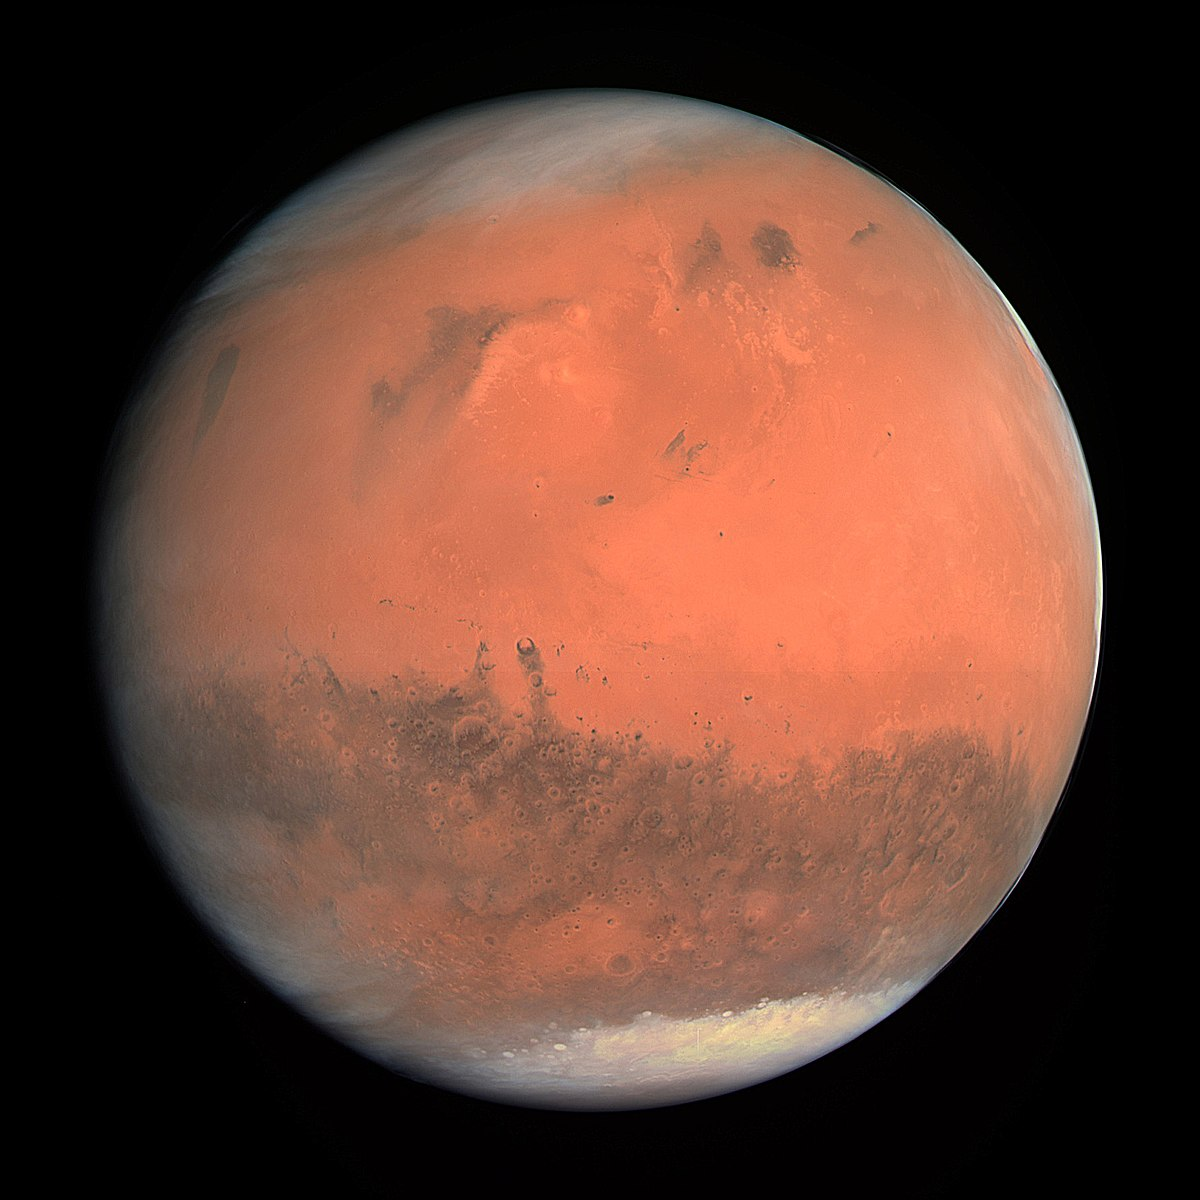
\includegraphics[width=1.0\textwidth]{Chapter2/Figures/picture.jpg}
\caption[List of Figures Text]{Caption Text}Source: \cite{oestereich2012analyse}.
\label{fig:picture1}
\end{figure}

\subsection{subsection1}

Lorem ipsum dolor sit amet, consectetur adipiscing elit, sed do eiusmod tempor incididunt ut labore et dolore magna aliqua. Ut enim ad minim veniam, quis nostrud exercitation ullamco laboris nisi ut aliquip ex ea commodo consequat. Duis aute irure dolor in reprehenderit in voluptate velit esse cillum dolore eu fugiat nulla pariatur. Excepteur sint occaecat cupidatat non proident, sunt in culpa qui officia deserunt mollit anim id est laborum.

\subsection{subsection2}

Lorem ipsum dolor sit amet, consectetur adipiscing elit, sed do eiusmod tempor incididunt ut labore et dolore magna aliqua. Ut enim ad minim veniam, quis nostrud exercitation ullamco laboris nisi ut aliquip ex ea commodo consequat. Duis aute irure dolor in reprehenderit in voluptate velit esse cillum dolore eu fugiat nulla pariatur. Excepteur sint occaecat cupidatat non proident, sunt in culpa qui officia deserunt mollit anim id est laborum. Lorem ipsum dolor sit amet, consectetur adipiscing elit, sed do eiusmod tempor incididunt ut labore et dolore magna aliqua. Ut enim ad minim veniam, quis nostrud exercitation ullamco laboris nisi ut aliquip ex ea commodo consequat. Duis aute irure dolor in reprehenderit in voluptate velit esse cillum dolore eu fugiat nulla pariatur. Excepteur sint occaecat cupidatat non proident, sunt in culpa qui officia deserunt mollit anim id est laborum.

\begin{figure}[h] 
\centering    
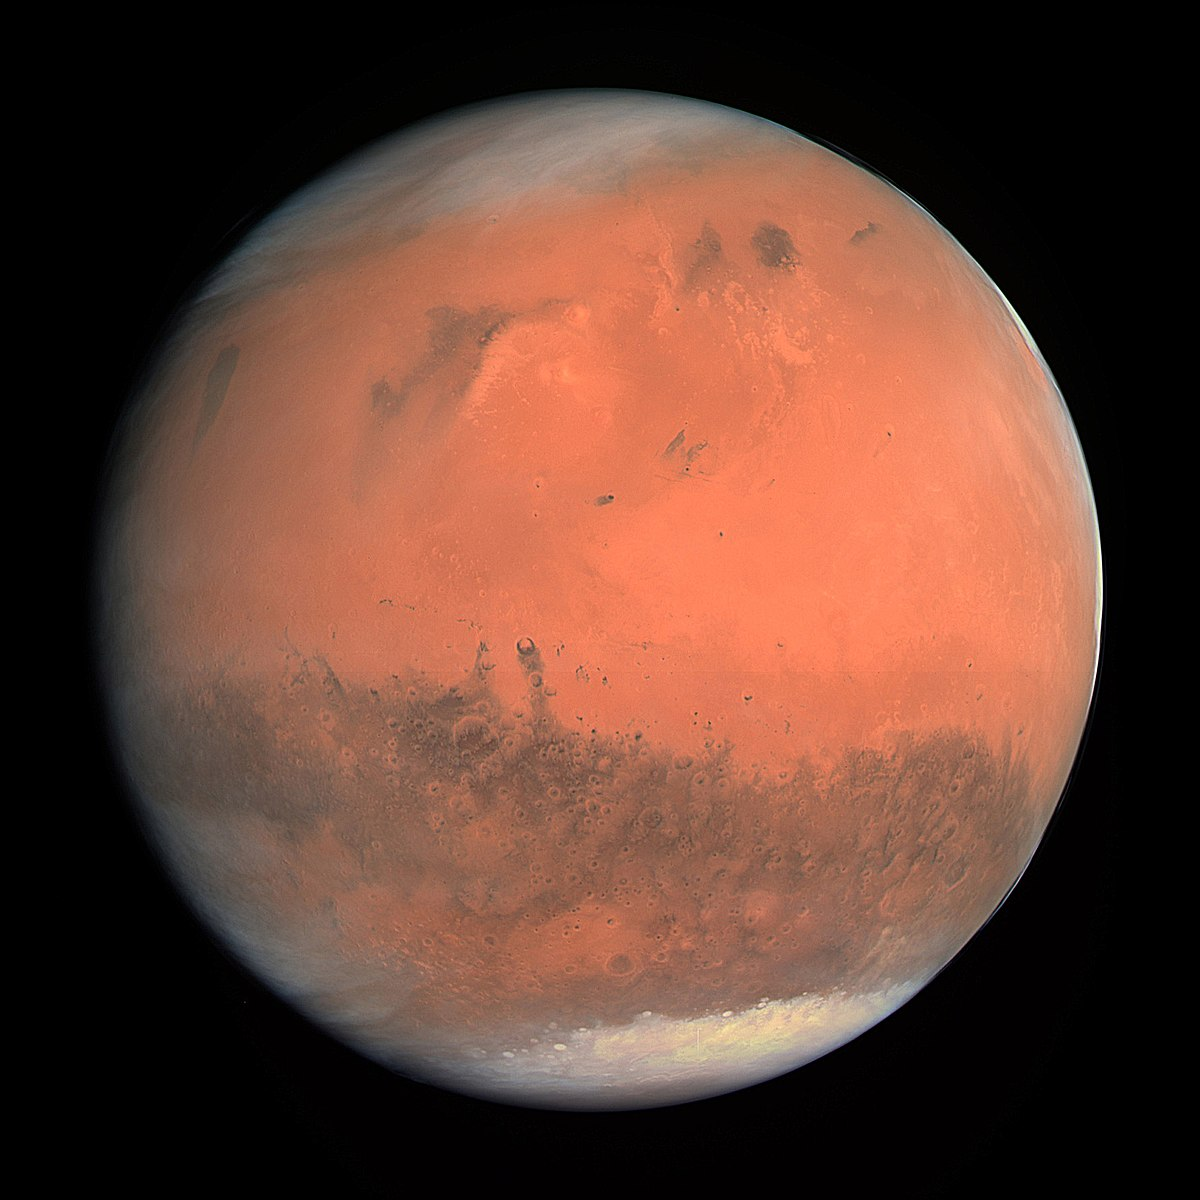
\includegraphics[width=1.0\textwidth]{Chapter2/Figures/picture.jpg}
\caption[List of Figures Text]{Caption Text2 Source: \citep{silver2016mastering}.}
\label{fig:picture2}
\end{figure}

\section{section2}
\label{sec:problemstellung}

Lorem ipsum dolor sit amet, consectetur adipiscing elit, sed do eiusmod tempor incididunt ut labore et dolore magna aliqua. Ut enim ad minim veniam, quis nostrud exercitation ullamco laboris nisi ut aliquip ex ea commodo consequat. Duis aute irure dolor in reprehenderit in voluptate velit esse cillum dolore eu fugiat nulla pariatur. Excepteur sint occaecat cupidatat non proident, sunt in culpa qui officia deserunt mollit anim id est laborum.

\begin{table}
\caption{Even better looking table using booktabs}
\centering
\label{table:good_table}
\begin{tabular}{l c c c c}
\toprule
\multirow{2}{*}{Dental measurement} & \multicolumn{2}{c}{Species I} & \multicolumn{2}{c}{Species II} \\ 
\cmidrule{2-5}
  & mean & SD  & mean & SD  \\ 
\midrule
I1MD & 6.23 & 0.91 & 5.2  & 0.7  \\

I1LL & 7.48 & 0.56 & 8.7  & 0.71 \\

I2MD & 3.99 & 0.63 & 4.22 & 0.54 \\

I2LL & 6.81 & 0.02 & 6.66 & 0.01 \\

CMD & 13.47 & 0.09 & 10.55 & 0.05 \\

CBL & 11.88 & 0.05 & 13.11 & 0.04\\ 
\bottomrule
\end{tabular}
\end{table}

% chapter 2
\chapter{Chapter3} 
\label{sec:chapter3}

Lorem ipsum dolor sit amet, consectetur adipiscing elit, sed do eiusmod tempor incididunt ut labore et dolore magna aliqua. Ut enim ad minim veniam, quis nostrud exercitation ullamco laboris nisi ut aliquip ex ea commodo consequat. Duis aute irure dolor in reprehenderit in voluptate velit esse cillum dolore eu fugiat nulla pariatur. Excepteur sint occaecat cupidatat non proident, sunt in culpa qui officia deserunt mollit anim id est laborum.

\section{section1}
\label{sec:hinführungzumthema}

Lorem ipsum dolor sit amet, consectetur adipiscing elit, sed do eiusmod tempor incididunt ut labore et dolore magna aliqua. Ut enim ad minim veniam, quis nostrud exercitation ullamco laboris nisi ut aliquip ex ea commodo consequat. Duis aute irure dolor in reprehenderit in voluptate velit esse cillum dolore eu fugiat nulla pariatur. Excepteur sint occaecat cupidatat non proident, sunt in culpa qui officia deserunt mollit anim id est laborum.

\subsection{subsection1}

Lorem ipsum dolor sit amet, consectetur adipiscing elit, sed do eiusmod tempor incididunt ut labore et dolore magna aliqua. Ut enim ad minim veniam, quis nostrud exercitation ullamco laboris nisi ut aliquip ex ea commodo consequat. Duis aute irure dolor in reprehenderit in voluptate velit esse cillum dolore eu fugiat nulla pariatur. Excepteur sint occaecat cupidatat non proident, sunt in culpa qui officia deserunt mollit anim id est laborum.

\begin{table}
\caption{Even better looking table using booktabs}
\centering
\label{table:good_table}
\begin{tabular}{l c c c c}
\toprule
\multirow{2}{*}{Dental measurement} & \multicolumn{2}{c}{Species I} & \multicolumn{2}{c}{Species II} \\ 
\cmidrule{2-5}
  & mean & SD  & mean & SD  \\ 
\midrule
I1MD & 6.23 & 0.91 & 5.2  & 0.7  \\

I1LL & 7.48 & 0.56 & 8.7  & 0.71 \\

I2MD & 3.99 & 0.63 & 4.22 & 0.54 \\

I2LL & 6.81 & 0.02 & 6.66 & 0.01 \\

CMD & 13.47 & 0.09 & 10.55 & 0.05 \\

CBL & 11.88 & 0.05 & 13.11 & 0.04\\ 
\bottomrule
\end{tabular}
\end{table}

\subsection{subsection2}

Lorem ipsum dolor sit amet, consectetur adipiscing elit, sed do eiusmod tempor incididunt ut labore et dolore magna aliqua. Ut enim ad minim veniam, quis nostrud exercitation ullamco laboris nisi ut aliquip ex ea commodo consequat. Duis aute irure dolor in reprehenderit in voluptate velit esse cillum dolore eu fugiat nulla pariatur. Excepteur sint occaecat cupidatat non proident, sunt in culpa qui officia deserunt mollit anim id est laborum.

\section{section2}
\label{sec:problemstellung}

Lorem ipsum dolor sit amet, consectetur adipiscing elit, sed do eiusmod tempor incididunt ut labore et dolore magna aliqua. Ut enim ad minim veniam, quis nostrud exercitation ullamco laboris nisi ut aliquip ex ea commodo consequat. Duis aute irure dolor in reprehenderit in voluptate velit esse cillum dolore eu fugiat nulla pariatur. Excepteur sint occaecat cupidatat non proident, sunt in culpa qui officia deserunt mollit anim id est laborum. Lorem ipsum dolor sit amet, consectetur adipiscing elit, sed do eiusmod tempor incididunt ut labore et dolore magna aliqua. Ut enim ad minim veniam, quis nostrud exercitation ullamco laboris nisi ut aliquip ex ea commodo consequat. Duis aute irure dolor in reprehenderit in voluptate velit esse cillum dolore eu fugiat nulla pariatur. Excepteur sint occaecat cupidatat non proident, sunt in culpa qui officia deserunt mollit anim id est laborum. Lorem ipsum dolor sit amet, consectetur adipiscing elit, sed do eiusmod tempor incididunt ut labore et dolore magna aliqua. Ut enim ad minim veniam, quis nostrud exercitation ullamco laboris nisi ut aliquip ex ea commodo consequat. Duis aute irure dolor in reprehenderit in voluptate velit esse cillum dolore eu fugiat nulla pariatur. Excepteur sint occaecat cupidatat non proident, sunt in culpa qui officia deserunt mollit anim id est laborum. Lorem ipsum dolor sit amet, consectetur adipiscing elit, sed do eiusmod tempor incididunt ut labore et dolore magna aliqua. Ut enim ad minim veniam, quis nostrud exercitation ullamco laboris nisi ut aliquip ex ea commodo consequat. Duis aute irure dolor in reprehenderit in voluptate velit esse cillum dolore eu fugiat nulla pariatur. Excepteur sint occaecat cupidatat non proident, sunt in culpa qui officia deserunt mollit anim id est laborum. Lorem ipsum dolor sit amet, consectetur adipiscing elit, sed do eiusmod tempor incididunt ut labore et dolore magna aliqua. Ut enim ad minim veniam, quis nostrud exercitation ullamco laboris nisi ut aliquip ex ea commodo consequat. Duis aute irure dolor in reprehenderit in voluptate velit esse cillum dolore eu fugiat nulla pariatur. Excepteur sint occaecat cupidatat non proident, sunt in culpa qui officia deserunt mollit anim id est laborum. Lorem ipsum dolor sit amet, consectetur adipiscing elit, sed do eiusmod tempor incididunt ut labore et dolore magna aliqua. Ut enim ad minim veniam, quis nostrud exercitation ullamco laboris nisi ut aliquip ex ea commodo consequat. Duis aute irure dolor in reprehenderit in voluptate velit esse cillum dolore eu fugiat nulla pariatur. Excepteur sint occaecat cupidatat non proident, sunt in culpa qui officia deserunt mollit anim id est laborum. Lorem ipsum dolor sit amet, consectetur adipiscing elit, sed do eiusmod tempor incididunt ut labore et dolore magna aliqua. Ut enim ad minim veniam, quis nostrud exercitation ullamco laboris nisi ut aliquip ex ea commodo consequat. Duis aute irure dolor in reprehenderit in voluptate velit esse cillum dolore eu fugiat nulla pariatur. Excepteur sint occaecat cupidatat non proident, sunt in culpa qui officia deserunt mollit anim id est laborum.

\begin{figure}[h] 
\centering    
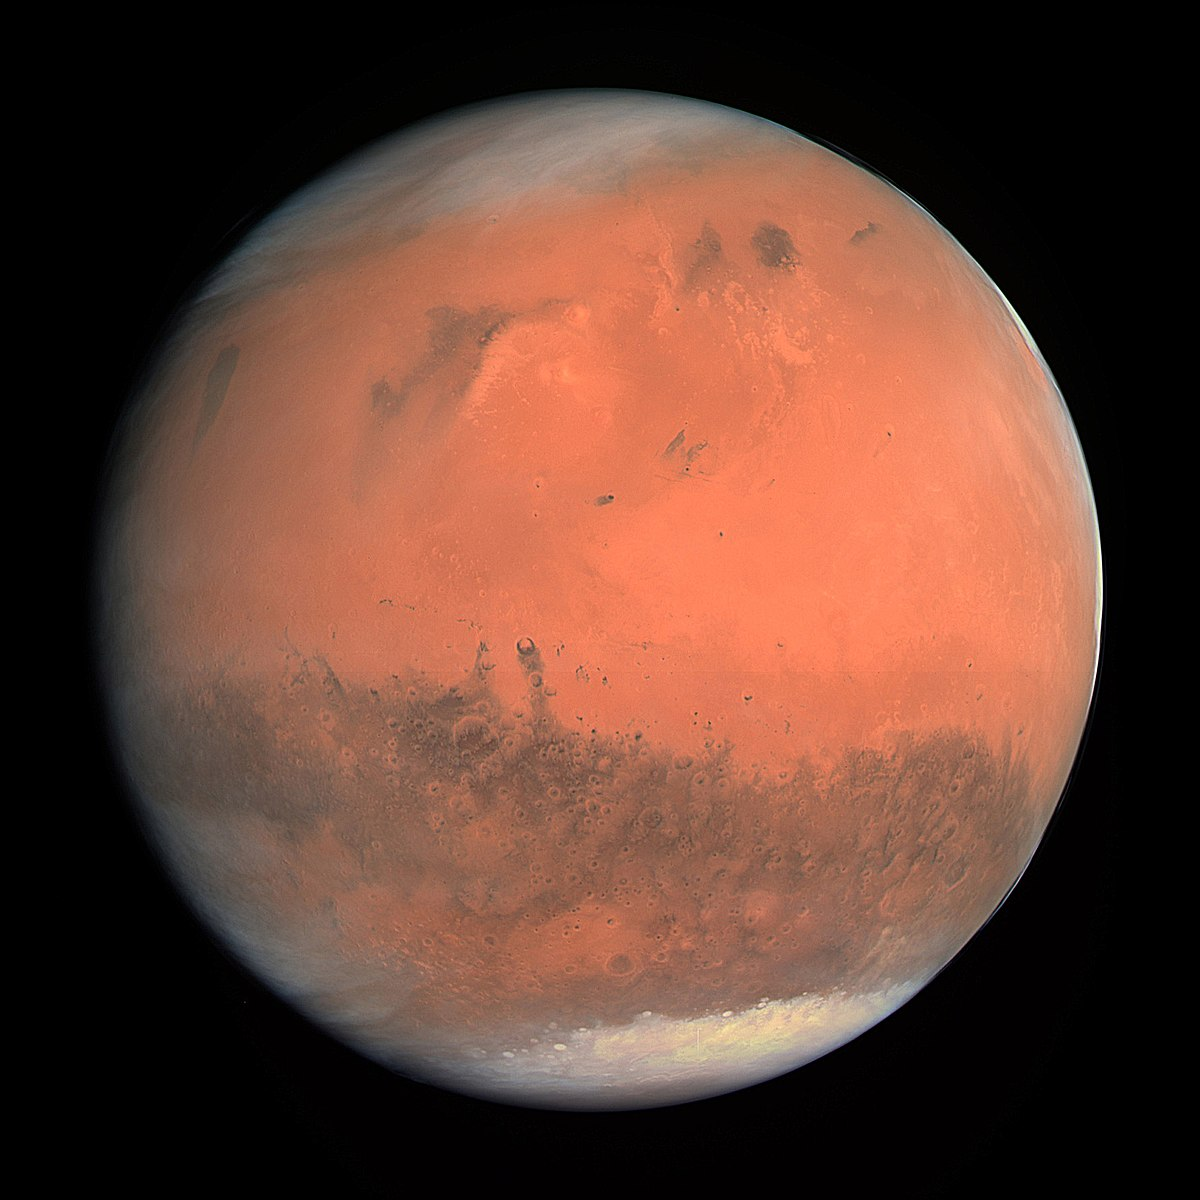
\includegraphics[width=1.0\textwidth]{Chapter2/Figures/picture.jpg}
\caption[List of Figures Text]{Caption Text}Source: Some Source .
\label{fig:picture3}
\end{figure}

% appendix
\appendix
\chapter{Appendix}
Lorem ipsum dolor sit amet, consectetur adipiscing elit, sed do eiusmod tempor incididunt ut labore et dolore magna aliqua. Ut enim ad minim veniam, quis nostrud exercitation ullamco laboris nisi ut aliquip ex ea commodo consequat. Duis aute irure dolor in reprehenderit in voluptate velit esse cillum dolore eu fugiat nulla pariatur. Excepteur sint occaecat cupidatat non proident, sunt in culpa qui officia deserunt mollit anim id est laborum.
\section{Section1}
Lorem ipsum dolor sit amet, consectetur adipiscing elit, sed do eiusmod tempor incididunt ut labore et dolore magna aliqua. Ut enim ad minim veniam, quis nostrud exercitation ullamco laboris nisi ut aliquip ex ea commodo consequat. Duis aute irure dolor in reprehenderit in voluptate velit esse cillum dolore eu fugiat nulla pariatur. Excepteur sint occaecat cupidatat non proident, sunt in culpa qui officia deserunt mollit anim id est laborum.
\section{Section2}
Lorem ipsum dolor sit amet, consectetur adipiscing elit, sed do eiusmod tempor incididunt ut labore et dolore magna aliqua. Ut enim ad minim veniam, quis nostrud exercitation ullamco laboris nisi ut aliquip ex ea commodo consequat. Duis aute irure dolor in reprehenderit in voluptate velit esse cillum dolore eu fugiat nulla pariatur. Excepteur sint occaecat cupidatat non proident, sunt in culpa qui officia deserunt mollit anim id est laborum.
\subsection{Subsection1}
Lorem ipsum dolor sit amet, consectetur adipiscing elit, sed do eiusmod tempor incididunt ut labore et dolore magna aliqua. Ut enim ad minim veniam, quis nostrud exercitation ullamco laboris nisi ut aliquip ex ea commodo consequat. Duis aute irure dolor in reprehenderit in voluptate velit esse cillum dolore eu fugiat nulla pariatur. Excepteur sint occaecat cupidatat non proident, sunt in culpa qui officia deserunt mollit anim id est laborum.
\subsection{Subsection2}
Lorem ipsum dolor sit amet, consectetur adipiscing elit, sed do eiusmod tempor incididunt ut labore et dolore magna aliqua. Ut enim ad minim veniam, quis nostrud exercitation ullamco laboris nisi ut aliquip ex ea commodo consequat. Duis aute irure dolor in reprehenderit in voluptate velit esse cillum dolore eu fugiat nulla pariatur. Excepteur sint occaecat cupidatat non proident, sunt in culpa qui officia deserunt mollit anim id est laborum.
\subsection{Subsection3}
Lorem ipsum dolor sit amet, consectetur adipiscing elit, sed do eiusmod tempor incididunt ut labore et dolore magna aliqua. Ut enim ad minim veniam, quis nostrud exercitation ullamco laboris nisi ut aliquip ex ea commodo consequat. Duis aute irure dolor in reprehenderit in voluptate velit esse cillum dolore eu fugiat nulla pariatur. Excepteur sint occaecat cupidatat non proident, sunt in culpa qui officia deserunt mollit anim id est laborum.

% bibliography
\clearpage
\addcontentsline{toc}{chapter}{References}
%\nocite{*}
\bibliography{References/references}{\protect\thispagestyle{plain}}
\renewcommand{\headrulewidth}{0pt}
\lhead{}
\chead{}
\rhead{}
\lfoot{}
\cfoot{}
\rfoot{\thepage}
\newpage

\end{document}